\documentclass{article}

\usepackage{fontspec}
\usepackage{array}
\usepackage{graphicx}
\usepackage{amsmath}
\usepackage{geometry}
\usepackage{amsmath}
\usepackage{algorithm}
\usepackage{algpseudocode}
\usepackage{subcaption} 
\newcommand{\myimagepath}{/Users/davidhodgson/Dropbox/Mac (3)/Documents/research/Rpackages/rjmc/}


\geometry{
    top=1in,
    bottom=1in,
    left=1in,
    right=1in,
}
\setmainfont{Avenir} 
\newcolumntype{M}[1]{>{\centering\arraybackslash}m{#1}}

%
\title{Modelling serological data using a reversible jump mcmc algorithm}
\author{David Hodgson}
\date{\today}

\begin{document}

\maketitle

\section{Overview of serological modelling}

\subsection{Serological sampling}


\paragraph{}Serological samples, such as blood or serum, can be used to detect the presence of biomarkers produced by the immune system in response to a specific pathogen.  This allows researchers and healthcare professionals to deduce crucial information about the epidemiological of the pathogen on the individual and population-level which may otherwise be missed by active surveillance systems.

\paragraph{}On the individual-level, serological samples can be used to determine if an individual has been previously infected with a particular infectious agent, even if the symptoms have resolved or were asymptomatic. After measuring the quantity of antibodies to a specific pathogen or pathogen, infection is usually inferred using an antibody threshold or by a threshold fold-rise between a pair of samples. In addition, researchers can study the specific immune responses generated by individuals during infection and see how they change according to certain host factors. This information can lead to a better understanding of the immune system's ability to combat various pathogens, aiding in the development of new treatments and vaccines. Studying Disease Dynamics: Serological data can provide insights into the transmission dynamics of infectious diseases. By analyzing changes in antibody prevalence over time, researchers can track the spread of a disease, identify hotspots, and better understand how pathogens move through populations.

\paragraph{}On the population-level, serological samples which are representative of a population, researchers can by used to estimate the prevalence of a specific infectious disease within that community. This information is invaluable for public health planning, resource allocation, and understanding the burden of a disease in a given region. In addition, serological tests can help assess the level of immunity within a population. This information is essential for designing vaccination campaigns, identifying vulnerable groups, and evaluating the effectiveness of vaccination programs. It also aids in making informed decisions during disease outbreaks. Finally, serological samples can be used to evaluate the effectiveness of vaccines by measuring the presence and levels of specific antibodies in vaccinated individuals. This data helps determine if a vaccine is providing adequate protection against the targeted pathogen and if booster shots are necessary.


\paragraph{}Serological samples play a pivotal role in understanding infectious diseases by providing information about past infections, disease prevalence, immunity levels, vaccine efficacy, and disease dynamics. They play an increasingly important role in public health efforts to combat and control infectious diseases. However, inferring infection requires a derivation of a abosolute or relative thresholdhold value however this is often determined heuristics (e.g. flu), but is highly variable between individuals. Consequently, better understanding of the kinetics of antibody trajectories post vaccination and infection can provide a better understanding of the heuristics used to infer infections from serological samples

\subsection{Antibody kineitcs}

\paragraph{}Modeling antibody kinetics involves using mathematical and statistical techniques to understand dynamics of antibodies in response to an infection or vaccination. Typically this involves the use of mathematical equations and statistical methods to describe the time-dependent changes in antibody levels within an individual or a population. Key components of such models include:
This process is essential for understanding how antibodies develop, peak, decline, and potentially provide protection against infectious diseases. Several attemps have been made to understand the kinetics of antibody kinetics, typically it follows a three stage process

\begin{itemize}
\item Initial Response: Modeling often starts by capturing the initial antibody response to a pathogen or vaccine. This phase is characterized by a rapid increase in antibody levels as the immune system recognizes and mounts a defense against the antigen.

\item vPeak Antibody Level: The models track the peak antibody level, which is the highest concentration of antibodies reached during the immune response. This peak can vary depending on factors like the strength of the immune response and the nature of the antigen.

\item Decay Phase: Antibody kinetics models also account for the decline in antibody levels following the peak response. Antibodies have a finite lifespan in the bloodstream, and their concentration gradually decreases as the pathogen is cleared or the vaccine antigen wanes.
\end{itemize}


\paragraph{}Modeling antibody kinetics provides several important benefits. First, by understanding the rate of antibody decline, models can estimate how long an individual's immunity is likely to last after infection or vaccination. This information is critical for designing vaccination schedules and determining the need for booster shots and permits the creation of better heuristics for determining infections using serology. Models help in understanding how changes in antibody levels impact disease transmission dynamics. This is vital for predicting and controlling outbreaks.


\paragraph{}Kinetics are also useful for optimizing vaccination strategies and can help identify the optimal timing and frequency of booster vaccinations to maintain protective antibody levels within a population. This is especially important for vaccine-preventable diseases with varying levels of immunity. Models allow researchers to evaluate the effectiveness of vaccines by comparing predicted antibody responses to observed data. This assessment aids in vaccine development and refinement.


\paragraph{}In conclusion, modeling antibody kinetics is a valuable tool for understanding the dynamics of immune responses to infections and vaccinations. It provides insights into immunity duration, vaccine efficacy, and strategies for disease prevention and control, ultimately contributing to better public health outcomes.

\subsection{Correlates of protection}
\paragraph{} Determining correlates of protection for infectious diseases is crucial for vaccine development and public health planning, but it can be challenging due to several factors. Here, we'll explore both the importance and the difficulties associated with identifying these correlates. Correlates of protection help researchers understand the specific immune responses needed to prevent or control an infectious disease. This knowledge is pivotal in designing and optimizing vaccines that can effectively induce the required immune response.

\paragraph{} Correlates also serve as critical benchmarks in assessing the effectiveness of vaccines during clinical trials. They allow researchers to measure whether a vaccine candidate can generate the necessary immune response and provide protection against the disease. By identifying correlates of protection informs vaccination strategies, including dosing schedules and target populations. It ensures that vaccines are administered optimally to achieve and maintain immunity, thus preventing outbreaks. Finally, understanding correlates of protection aids in devising strategies for controlling and eventually eradicating infectious diseases. By targeting specific immune responses, interventions can be more effective.

\paragraph{}Determining whether someone has been exposed to an infection but protected due to existing antibody levels is key in determining correlates of protection. Those who have been infected have also been exposed, but those who do not acquire infection detectable by antibodies, or the infection is aborted by other immune processes, are particularly difficult to detected with out without intense contact tracing which is challanging and difficult to roll-out on a large scale, or intense immune profiling. Further diseases may require unique approaches, and not all diseases have well-established correlates. Existing correlates have been determined through Challenge Studies: In controlled challenge studies, volunteers are deliberately exposed to the pathogen after vaccination. Researchers monitor their immune responses and assess whether they remain protected or develop the disease. This approach allows for a direct evaluation of correlates of protection. However these are expensive and determine. 


\paragraph{}In conclusion, determining exposure to infections in a population is vital for public health efforts, but it comes with significant challenges, including asymptomatic cases, testing limitations, and the complexities of immune responses. Overcoming these challenges requires a combination of improved testing strategies, data collection, and the continued development of diagnostic tools to ensure accurate and timely identification of exposed individuals.

\subsection{Determining correlates of protection and antibody kinetics in a single framework}
\paragraph{}To overcome the issues of biasing antibody kinetics due to lack of informatin on exposure, we present a single framework which takes individual-level serological sample data and uses changes in antibody titres over time to determine i) the subsequent antibody kinetics of these infection individuals and ii) the correlate of protection preventing exposued individuals from becoming infected. The intermeidate process which allows this is a process which determines exposed and individuals who are infected with the virus, into a single mathematical framework we can properly quantifythe uncertainty in the framework by allows interdependencies between these modules (i.e. antibody kinetics, those infected) and provide more accurate understanding of the serological inference with out the need for pre-determined heureistics. 

\subsection{Simulated data}
\paragraph{}To explain the framework we simulate serological data using the \texttt{serosim}[ref] R package. We simulate continuous epidemic serosurveillence (CES) cohort data, but we also provide information in the appendix for pre- and post-pandemic serosurvey (PPES) cohort data. CES data represents a study in which individuals are followed over a period spanning an epidemic wave and bled at multiple random time points throughout. The simulated data includes 200 individuals with serological samples taken within the first seven days of the study's starting and a sample within the last seven days of the study's ending. These individuals also had three samples taken randomly throughout the study (over the 120-day epidemic wave). Each individual has a 60\% chance of exposure to the virus over the study timeframe. To model an even epidemic peak, we simulate the exposure rate for each individual from a normal distribution, $N(60, 20)$. 



\paragraph{}The correlate of protection is the probability of infection given a titre value at exposure. Two different sets of data are simulated with two different correlates of protection; one is uniform for all titres at exposure and thus represents no correlation of protection. The second follows a logistic distribution of the form:

\begin{equation}
\label{eq_cop}
f_{cop}(z, \beta_0, \beta_1) = \frac{1}{1 + \exp(- (\beta_0 + \beta_1z))}
\end{equation}

where $\beta_0 = 2$ and $\beta_1 = 2$ in the simulated data. This represents a pathogen for which higher antibody titres are associated with higher levels of protection from infection.

\paragraph{}The antibody kinetics are assumed to follow a linear rise to a peak at 14 days, followed by an exponential decay to a set=piont value as defined in X[ref]. The formula for this biphasic trajectory is given by Equation~\ref{eq_ab}

\begin{equation}
\label{eq_ab}
F_{ab}(s, a, b, c) =
\begin{cases}
  \ln(\exp(a) + \exp(b)) / 14, & \text{if }s \leq 14 \\
  \ln(\exp(a) \exp(-(b/10)(t - 14)) + \exp(c)), &\text{if } s > 14
\end{cases}
\end{equation}

where $a = 1.5$, $b = 2$, and $c = 1$ are values in the simulated data (Figure) and $s$ is the number of days post infection. We also assume that the magnitude of these dynamics are dependent on pre-existing titre value, with higher pre-existing values seeing attenuated dynamics relative to lower pre-existing tire values. The titre dependent boosting is assumed to follow a linear decay truncated at 0, that is, given a titre value $z$, $f_{tp}(z, \alpha) = \max(1 - \alpha z, 0)$. where $\alpha = 0.3 $ in the simulated data.  Therefore the value to the value depends on the time $t$ and titre value at infection $z$;  

\begin{equation}
\label{eq_ab2}
f_{ab}(s, z, a, b, c, \alpha) = F_{ab}(s, a, b, c)f_{tp}(z, \alpha) 
\end{equation}

\begin{figure}[ht]
    \centering
    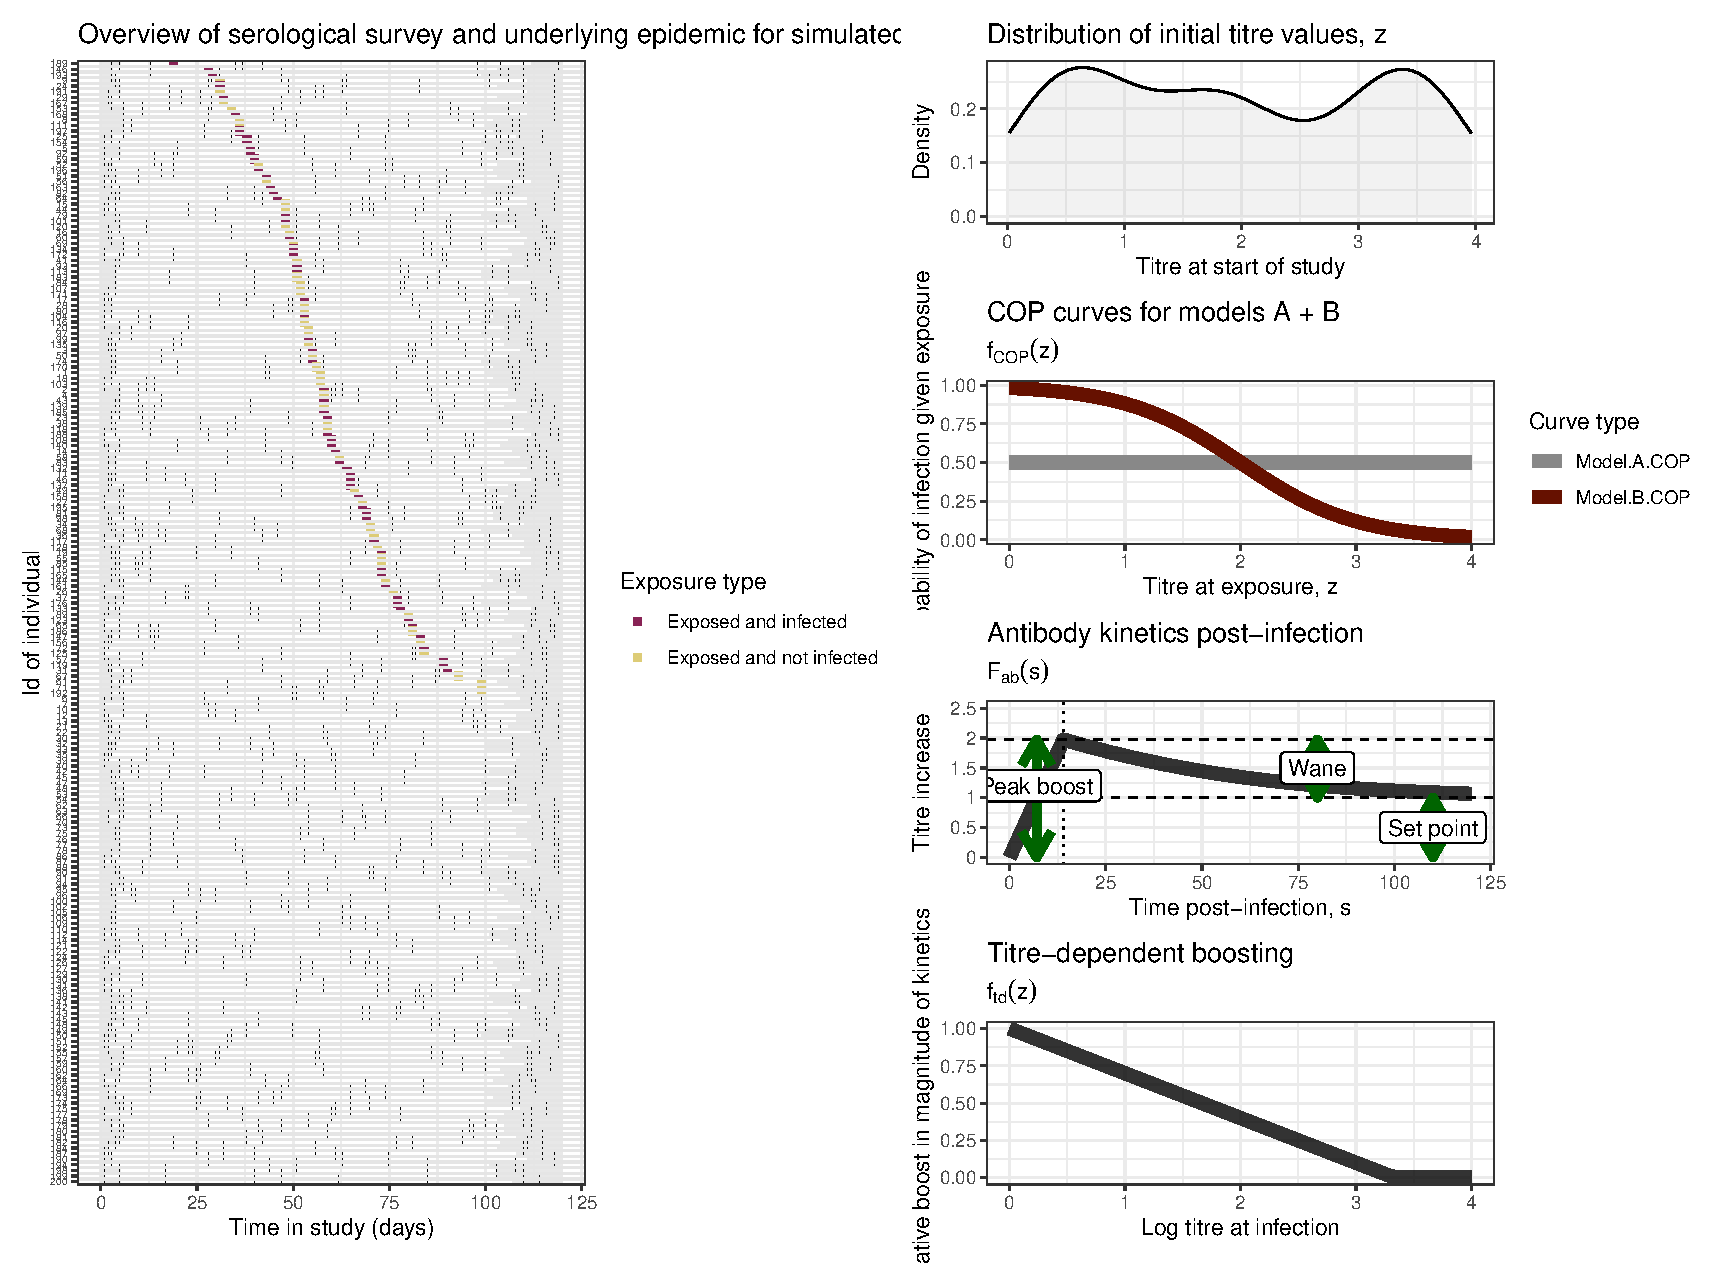
\includegraphics[width=1\textwidth]{\myimagepath/outputs/sim_data/summary_fig_A_CES.pdf}     \caption{Schematics showing the simulated data structure from \texttt{serosim}[ref]}
    \label{fig:sim_A}
\end{figure}



\paragraph{}To model individual-level in antibody kinetics, capturing both indiviudal hetergeneity in repsonses nad. measurement uncertaity, we simulate responses with for $a, b, c, \alpha$ from a normal distributions centered at where X is chosen. We simulate three  llevels of uncetainty, 0.01, 0.2, 0.5 for each correlate of protection model, giving six datasets in total. A schematic showing how the variance influences the trajectories of a variability of the antibody kinetics is shown in Figure X. 

\begin{figure}[ht]
    \centering
    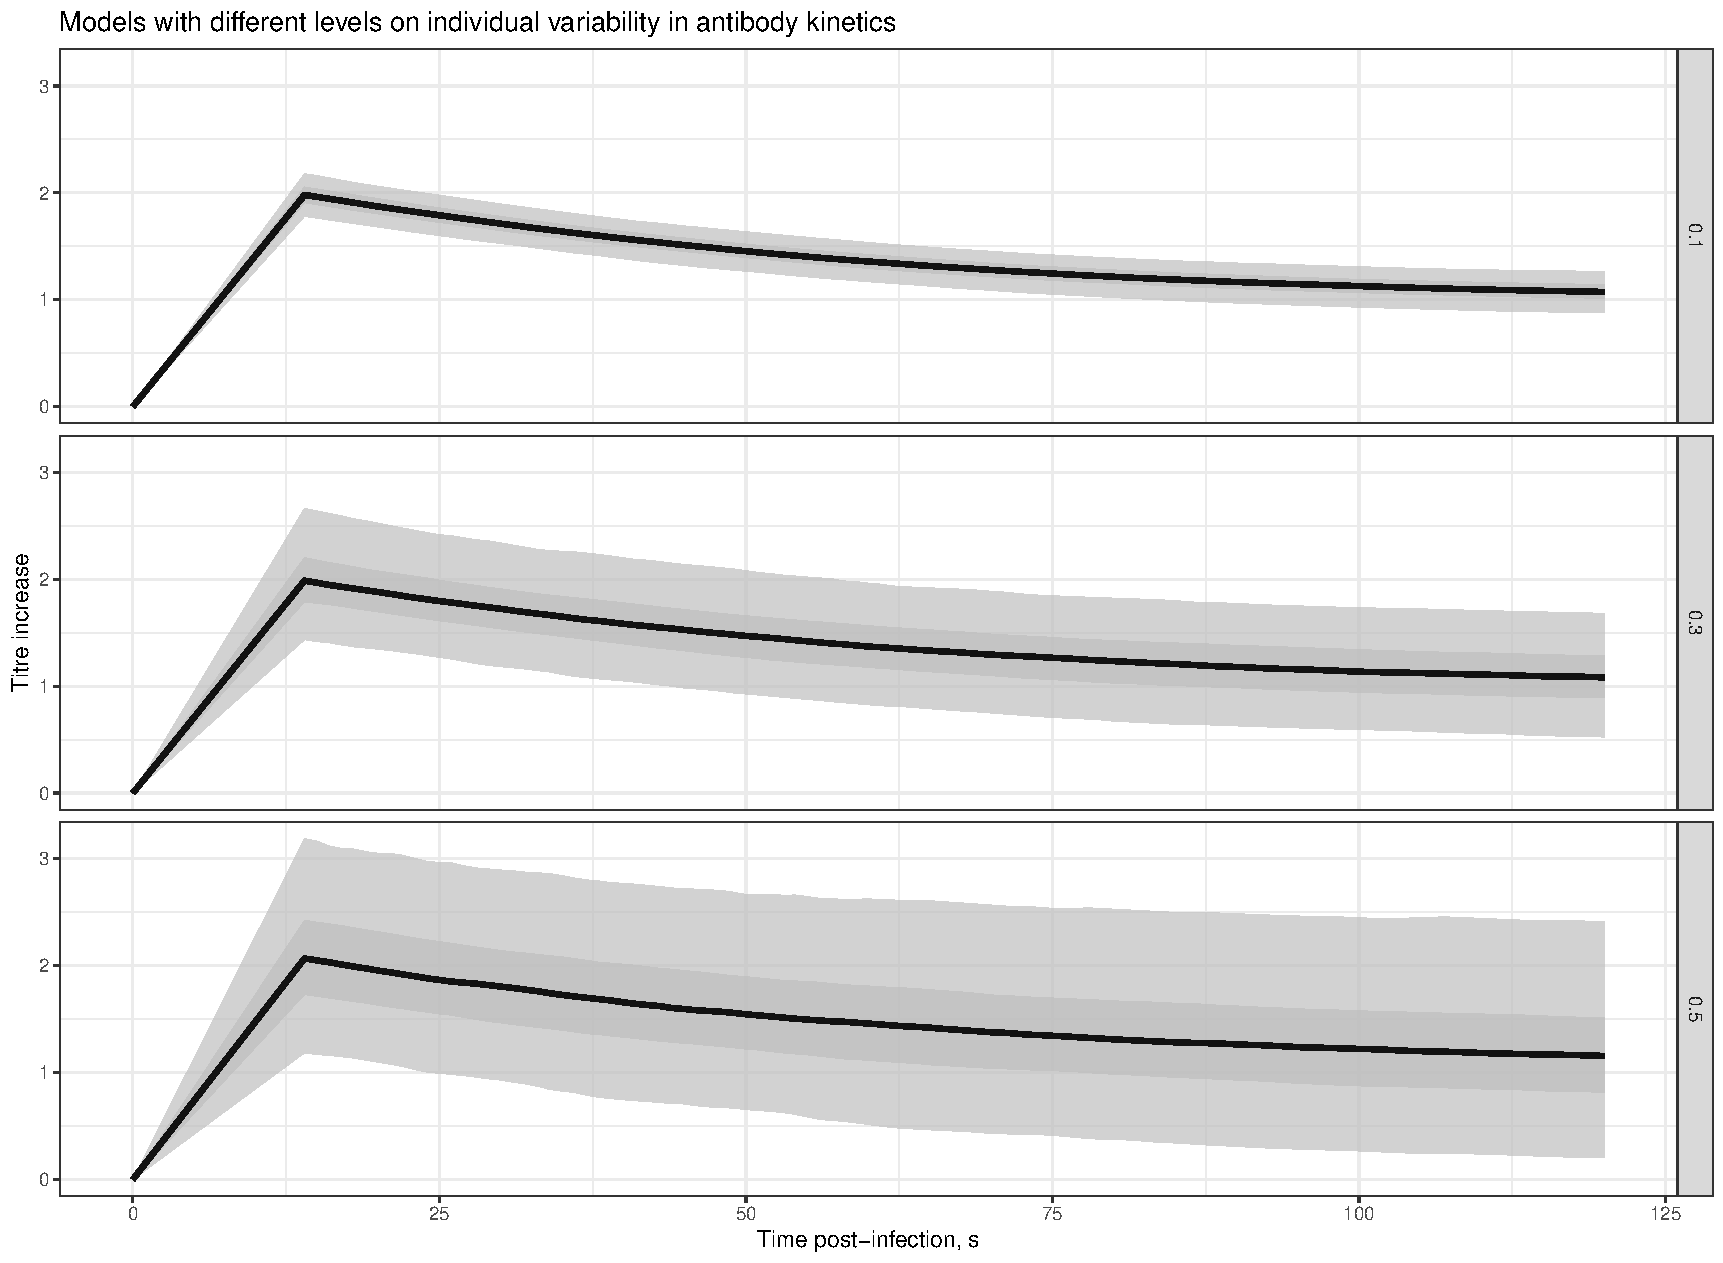
\includegraphics[width=1\textwidth]{\myimagepath/outputs/sim_data/summary_fig_B_CES.pdf}     \caption{Schematics showing three levels of individual-level uncertainty and the impact on the  variability of antibody kinetics.   }
    \label{fig:sim_B}
\end{figure}

\paragraph{}For these six simulated data sets, information on the number exposed and infected is given in Table X. We will fit the to-be-described methods to these datasets and explore how the correlation of protection and level of variability in in antibody kinetics impacts the framework's ability to recovery simulated data. 





\newpage
\section{Inference with known exposure status}

\paragraph{}We now provide a methodological walkthrough for how the reversible-jump mcmc serological (RJMCMC) framework works. First, we will show simulation recovery in a pedagogical case in which we assume the time of exposure and exposure status is known. Though this is not possible in practice, this example will help explain how the MCMC sampler works without having to describe the more complex RJMCMC. We show that the correlate of protection and antibody kinetic s are well recovered. In the second section, we show assume that exposure status and time is not known for each indivdual, and describe how the  RJMCMC framework works. We find that the timing and exposure, infection status, correlation of protection and antibody kinetics are recovered for our simulated data.

\subsection{Mathematical representation}

For each individual, $i$, has three states that must be inferred, $E_i$, whether they are exposed over the study period, $E_i^t$ the timing of their exposure, $I_i$ whether they are infected (Table~\ref{ab:states}).

\begin{table}[ht]
\label{tab:states}
    \centering
    \caption{Inferrable epidemiological states}
     \resizebox{\textwidth}{!}{%
      \tiny 
    \begin{tabular}{|p{2cm}|p{4cm}|p{6cm}|}
        \hline
          \rule{0pt}{0.5cm}\textbf{Symbol} &  \textbf{Description}  & \textbf{Values}\\
        \hline
      $E_i$ & Exposure status of individual $i$ & Binary value. 0: Not exposure, 1: exposed. \\
        \hline
        $E^t_i$ & Time of exposure for individual $i$  & Continuous value between start of study ($T = 0$) and values of study ($T = T_{end}$) \\
        \hline
        $I_i$ & Infection status of individual $i$. & Binary value. 0: Not infected, 1: Infected. \\
        \hline
    \end{tabular}
    }
\end{table}

For example, a person who is not exposed has values E = 0, E = NA, and I is always 1. For E = 1, E = 60 days (after the start of the study), and I is either 0 or 1, depending on the protection correlation. In this example, we know the value of $E_i$ and $E_i^t$ for each individual. Thus we need only infer the status of $I$. 

\paragraph{}We first define several functions which will help us calculate our likelihood. First, we assume that the model predicted antibody titre at time $t$ in the study ($X_{i.t}$) can be derived given the infection status $I_i$ and timing of exposure $E_i^t$. If a person is not infected, then their starting titre value ($Z^0_i$) remains unchanged from the state of the study. If the person is infected, their titre remains unchanged until the point of infection, at which point they follow the dynamics highlighted in Eq[]. The deterministic function for calculating this value is given by

\begin{equation}
\label{eq:ll_abkin}
X_{i,t}  = P_{ab}( I_i,  E_i^t, a, b, c, \alpha, Z^0_i) = 
	\begin{cases}
	Z^0_i, & \text{If $I_i = 0$ or $E_i = 0$ or if $E_i^t > t$} \\ 
	Z^0_i + f_{ab}(t - E_i^t, Z^0_i,  a, b, c,  \alpha),  & \text{Otherwise} \\
	\end{cases}
\end{equation}


Second, we define a likelihood function for the correlation of protection. For an individual $i$, with $E_i = 1$, the correlate of protection given exposure at time $t$ with titre value $X_{i.t}$, given by a Bernoulli distribution with the probability is given by X
\begin{equation}
\label{eq:ll_cop}
P_{cop}(I_i \mid E_i = 1, X_{i.t}, \beta_0, \beta_1) =  f_{cop}(X_{i.t},  \beta_0, \beta_1)^{I_i}(1- f_{cop}(X_{i.t},  \beta_0, \beta_1))^{1-I_i}
\end{equation}

\paragraph{}Finally, we define an observational model to capture variability between hosts and measurement error. Assuming that the model predicted titre value at time $t$ for individual $i$ is given by, $X_{i.t}$ and the serologicla antibody body at the same time point is given by $Z_{i.t}$, we assume the measrement error follow a normal distribution and dervied the following likliehood.

\begin{equation}
\label{eq:ll_obs}
P_{obs}(Z_{i,t} \mid X_{i.t}, \sigma) = \frac{1}{\sigma \sqrt{2\pi}} \, e^{-\frac{(Z_{i,t} - X_{i.t})^2}{2\sigma^2}}
\end{equation}

where $\sigma$ is fitted in the model. We let $\theta = \{a,b, c, \alpha, \beta_0, \beta_1\}$ for clarity henceforth. 


\subsection{Posterior distribution via Bayes rule}

We have two different posterior distributions depending on whether an individual is exposed ($E_i = 1$) or not ($E_i = 0$).

\subsubsection{Case 1. $E_i = 0$} 
In this case the value of the timing of exposure is not applicable and the individual cannot have been infected (i.e. $E^t_i = \text{NA}, I_i = 0)$. The likelihood  for this individual with serological samples taken at times $t\in T$ is therefore equivalent to:
\begin{equation}
L_{E_i = 0}(Z_{i}| \theta) = \prod_{t \in T}P_{obs}(Z_{i,t}|Z^0_{i}, \sigma)
\end{equation}
as $X_{i.t} = Z^0_{i}$ for all $t$.



\subsubsection{Case 2. $E_i = 1$}
In this case, the value of the timing of exposure is taken from a user-defined probability distribution approximated to the epidemic curve ($f_I$), and the infectious status is determined by the correlate of protection function ($f_{cop}$). (i.e. $E^t_i = \text{NA}, I_i = 0)$. The likelihood for this individual with serological samples taken at times $t\in T$ and infection time $\tau$ is therefore equivalent to:

\begin{equation}
L_{E_i = 1}(Z_{i}| I_i, \theta) = \prod_{t \in T}P_{obs}(Z_{i,t}|X_{i,t}, \sigma)P_{cop}(I_i \mid  X_{i.t}, \theta)
\end{equation}

where $X_{i,t} =P_{ab}( I_i,  E_i^t, a, b, c, \alpha, Z^0_i) $.


\subsubsection{Total likelihood}
If $N_{E=0}$ and $N_{E = 1}$ is the set of individuals which are not exposure and exposed respectively, then the total likelihood can be written 
\begin{equation}
L(Z|I, N_{E=0}, N_{E=1}, \theta) = \prod_{i \in N_{E=0}}L_{E_i = 0}(Z_{i}| \theta) \prod_{i \in N_{E=1}}L_{E_i = 1}(Z_{i}| I_i, \theta) 
\end{equation}

\subsubsection{Prior distributions}

\paragraph{}We choose prior distributions for each parameter \pi($\theta$). Table gives a summary of the priors we choose with the support. 

\begin{table}[ht]
    \centering
    \begin{tabular}{|l|l|l|}
        \hline
        \textbf{Parameter} & \textbf{Prior ($\pi$)} & \textbf{Support ($\mathcal{S}$)} \\
        \hline
        a & $\mathcal{N}(1.5, 0.5)$ & $[0.5, 4]$ \\
        \hline
        b & $\mathcal{N}(0.3, 0.05)$ & $[0, 1]$ \\
        \hline
        c & $\mathcal{U}(0, 4)$ & $[0, 4]$ \\
        \hline
        $\alpha$ & $\mathcal{U}(0, 1)$ & $[0, 1]$ \\
        \hline
        $\beta_0$ & $\mathcal{U}(-10, 10)$ & $[-10, 10]$ \\
        \hline
        $\beta_1$ & $\mathcal{U}(-10, 10)$ & $[-10, 10]$ \\
        \hline
        $\sigma$ &  $\mathcal{U}(0.01, 1)$ & $[0.01, 1]$ \\
        \hline
    \end{tabular}
    \caption{Table with Headers: Parameter, Prior, and Support}
    \label{tab:mytable}
\end{table}

\paragraph{}We also choose the prior for the number of infections $\mathcal{N}_I$ given the number of exposed individuals $\mathcal{N}_E$ to be a Beta Binomial distribution: $\pi(\mathbf{I}) = \text{BetaBinomial}(\mathcal{N}_I | \mathcal{N}_E, 1, 1)$. Choosing this prior prevents any implicit priors that might rise from products of Bernoullis(HAY) as $\text{BetaBinomial}(\mathcal{N}_E, 1, 1) = 1 / \mathcal{N}_E$, further in this example as $\mathcal{N}_E$ is fixed. Thus, this term cancels in the acceptance probability. 


\subsubsection{Posterior distributions}

\paragraph{}Bayes' rule stipulates that the product of the prior distribution and likelihood is proportional to the posterior distribution; we can use this rule to approximate the posterior for use in the metropolis algorithm. Specifically 

\begin{equation}
P(\theta, I | Z) \propto \mathcal{L}(Z | \theta, I)\pi(\theta)\pi(I)
\end{equation}


\subsection{Metropolis-Hasting algorithm}

\subsubsection{Overview}
\paragraph{} The Metropolis-Hastings algorithm is a widely used method for generating samples from a target probability distribution. It falls under the broader category of Markov Chain Monte Carlo (MCMC) methods and is particularly useful when direct sampling from the desired distribution is challenging or impossible such as the likelihood described above. The Metropolis-Hastings algorithm offers a solution to this problem. It is a Markov chain-based approach that iteratively generates a sequence of samples, which eventually converge to the desired distribution. 

\paragraph{}Say we wish to sample from an intractable probability distribttion $p(x)$. The idea of the MH is to define a Markov chain over possible values in such a way that the stationary distribution of the Markov chain is in fact $p(x)$. That is, the resulting Markov chain from MH generates a sequence of values, denoted $\{\theta_1, \theta_2, \dots,  \theta_n\}$, such that as $n -> \infty$ we can guarantee that $theta_i \sim p(x)$. The MH algorithm is a two part process, first a proposal value $\theta^*$ is sampled from a proposal distribution, $Q$, centered at the current chain step $\theta$, $\theta \sim Q(\theta)$. This proposal is then accept according to a acceptance ratio whichis the ratio of the posterior distribution evaluated at the newly sampled chain and the posterior distribution sampled at the current chain. A general algorithm is given in Algorithm~\ref{alg:metropolis_hastings}..
\begin{algorithm}
\caption{Generic Metropolis-Hastings Algorithm}
\label{alg:metropolis_hastings}
\begin{algorithmic}[1]
    \State Initialize the chain with an initial state $\theta_0$
    \For{$i = 1$ to $N$}
        \State Generate a candidate state $\theta'$ from the proposal distribution: $\theta' \sim Q(\theta_i)$
        \State Compute the acceptance ratio:
        \[
        \alpha = \min\left(1, \frac{P(\theta')}{P(\theta_i)} \cdot \frac{Q(\theta_i \mid \theta')}{Q(\theta' \mid \theta_i)}\right)
        \]
        \State Generate a uniform random number $u$ from the interval $[0, 1]$
        \If{$u \leq \alpha$}
            \State Accept the candidate state: $\theta_{i+1} \leftarrow \theta'$
        \Else
            \State Reject the candidate state: $\theta_{i+1} \leftarrow \theta_i$
        \EndIf
    \EndFor
\end{algorithmic}
\end{algorithm}

\subsubsection{MH for serological inference with known exposure }

\paragraph{}In our datasets we wish to infer $\theta$, and infectious statuses ${I_j} \in \mathcal{I}$, for $1 \leq j \leq M$ individuals. By letting $J_i \in(\theta_i, I_i)$) . For the proposal distribution, we define independent proposal distribution for each $\theta$ and $I_i$,  such that $Q(\theta_i, \mathcal{I}_i) = q_\theta(\theta)q_I(\mathcal{I}_i)$. The proposal distribution for $q_\theta(\theta_i, \theta_{i, adapt})$ is a multivariate normal distribution with an adaptive covariance matrix which requires a set of parameters to be updated at each time step $\theta_{i, adapt}$.[ref] (See Appendix). The proposal distribution for $q_I(\mathcal{I}_i)$, which is a discrete space, is performed by choosing an individual $j$ such that $E_i = 1$ uniformly, at each time step, $i$, then sampling a value for $I_{i, j} sim \text{Bernoulli(0.5)}$. These prosposal are both symmetric and thus cancel out in the acceptance ratio. Consequently, we edit the algorithm as given in Algorithm~\ref{alg:metropolis_hastings_inf}.

\begin{algorithm}
\caption{Metropolis-Hastings Algorithm for antibody kinetics and infection inference}
\label{alg:metropolis_hastings_inf}
\begin{algorithmic}[1]
    \State Initialize the chain with an initial state $\theta_0$ from the priors $\pi(\theta)$ and $I_{0, j} \sim \text{Bernoulli(0.5)}$ for all $M$ individuals and determine $\theta_{0, adapt}$.
    \For{$i = 1$ to $N$}
        \State Generate a candidate state $\theta' \sim q_\theta(\theta_i, \theta_{i, adapt})$
        \State Generate a candidate individual $j \in N_{E = 1} $ and then a candidate state $I'_j \sim \text{Bernoulli(0.5)}$
        \State Compute the acceptance ratio:
        \[
        \alpha = \min\left(1, \frac{P(\theta', I'_{j}|Z)}{P(\theta_i, I_{i, j}|Z)} \right)
        \]
        \State Generate a uniform random number $u$ from the interval $[0, 1]$
        \If{$u \leq \alpha$}
            \State Accept the candidate state: $\theta_{i+1} \leftarrow \theta'$ and $I_{i + 1, j}  \leftarrow I'_j$
        \Else
            \State Reject the candidate state: $\theta_{i+1} \leftarrow \theta_i$ and $I_{i + 1, j}  \leftarrow I_{i, j} $
        \EndIf 
        \State Update $\theta_{i + 1, adapt} \leftarrow \theta_{i, adapt}$
    \EndFor
\end{algorithmic} 
\end{algorithm}

\subsection{Implementation }
\paragraph{} We code the algorithm manually in cpp with an R interface. We run the algorithm for 200,000 steps, with 100,000 burn-in and for 4 chains. The starting value is taken from the prior distributions of the for $\theta$ and $I$ respectively. We initialise the adaptive covariance by running with an identity matrix with each parameter scale according to 1,000 steps, then sample from the adaptive scheme as in XX. 

\subsection{Simulation recovery }
\paragraph{} After running the algorithm, we demonstrate the ability of MH algorithm X to recover the simulated data derived in section X.

\subsubsection{Infection recovery}

\paragraph{}We assess the ability of the algorithm to recover the infection status of each individual in the study. If the set posterior samples of the infection status is given by $\hat{I_i}$, then we defined an inferred infection to be the case where 75\% or more samples are equal to 1, similarly we define a non-infection event for an individual to be the case were 75\% or are equal to 0. In the case where a individual is netiher infered to be infected or non-infected, we define their infection status as 'non-inferable'.  Given no COP, we find when the pre-infection titre < 3 that all six models considered are able to recover the infection status of all individuals exactly. When the pre-infection titre is greater than 3, the remaining samples are 'non-inferable'; this is due to the attenuation of boosting for infected individuals causing no meaningful change in ab-boosting, and thus, these infections are no longer inferable. In our COP model (model B) we find that the inclusion of the correlate of protection influence the inferrable infection status, causing all infection status, regardless of pre-infection titre to be recoverable. 

\begin{figure}[H]
    \centering
    \begin{subfigure}{0.31\textwidth}
        \centering
        \includegraphics[width=\textwidth]{\myimagepath/outputs/fits/cesNoCOP/knownExp/figs/obs_0/infection_recov.png}
        \caption{No COP, 0\% observation error}
    \end{subfigure}
    \begin{subfigure}{0.31\textwidth}
        \centering
        \includegraphics[width=\textwidth]{\myimagepath/outputs/fits/cesNoCOP/knownExp/figs/obs_0.2/infection_recov.png}
        \caption{No COP, 20\% observation error}
    \end{subfigure}
    \begin{subfigure}{0.31\textwidth}
        \centering
        \includegraphics[width=\textwidth]{\myimagepath/outputs/fits/cesNoCOP/knownExp/figs/obs_0.5/infection_recov.png}
        \caption{No COP, 50\% observation error}
    \end{subfigure}
    
  \begin{subfigure}{0.31\textwidth}
        \centering
        \includegraphics[width=\textwidth]{\myimagepath/outputs/fits/cesCOP/knownExp/figs/obs_0/infection_recov.png}
        \caption{ COP, 0\% observation error}
    \end{subfigure}
    \begin{subfigure}{0.31\textwidth}
        \centering
        \includegraphics[width=\textwidth]{\myimagepath/outputs/fits/cesCOP/knownExp/figs/obs_0.2/infection_recov.png}
        \caption{ COP, 20\% observation error}
    \end{subfigure}
    \begin{subfigure}{0.31\textwidth}
        \centering
        \includegraphics[width=\textwidth]{\myimagepath/outputs/fits/cesCOP/knownExp/figs/obs_0.5/infection_recov.png}
        \caption{ COP, 50\% observation error}
    \end{subfigure}
    
    \caption{Simulation recovery of infection status and epidemic curve for two COP models (top: No COP, bottom: logistic COP) and three different levels antibody kinetics variability (0, 20\%, 50\%)}
\end{figure}


\subsubsection{Correlate of protection}

\paragraph{}We next assess the ability of the MH Algorithm to recover the correlate of protection. WE consider two COP models; Model A, no correlate of protection, Model B; logsitical curve for COP. For cour No correlate model we find that the COP curve is most recovered, with the simulated line within a 50\% confidence interval of the posterior sample. Though the model seems to estimate higher change of protection at higher pre-infection values comopare to lower infection values. This is likle an artifact of both fitting a logsitical curve to a straight line which is intrinsically tricky and small sample size leading to biases at one extreme. for the COP model, we find the COP structure is recovered. The variability in the antibody kinetics seemed to have a negligible effect on the recoverability of the COP curve. 

\begin{figure}[H]
    \centering
    \begin{subfigure}{0.31\textwidth}
        \centering
        \includegraphics[width=\textwidth]{\myimagepath/outputs/fits/cesNoCOP/knownExp/figs/obs_0/cop_recov.png}
        \caption{No COP, 0\% observation error}
    \end{subfigure}
    \begin{subfigure}{0.31\textwidth}
        \centering
        \includegraphics[width=\textwidth]{\myimagepath/outputs/fits/cesNoCOP/knownExp/figs/obs_0.2/cop_recov.png}
        \caption{No COP, 20\% observation error}
    \end{subfigure}
    \begin{subfigure}{0.31\textwidth}
        \centering
        \includegraphics[width=\textwidth]{\myimagepath/outputs/fits/cesNoCOP/knownExp/figs/obs_0.5/cop_recov.png}
        \caption{No COP, 50\% observation error}
    \end{subfigure}
    
  \begin{subfigure}{0.31\textwidth}
        \centering
        \includegraphics[width=\textwidth]{\myimagepath/outputs/fits/cesCOP/knownExp/figs/obs_0/cop_recov.png}
        \caption{ COP, 0\% observation error}
    \end{subfigure}
    \begin{subfigure}{0.31\textwidth}
        \centering
        \includegraphics[width=\textwidth]{\myimagepath/outputs/fits/cesCOP/knownExp/figs/obs_0.2/cop_recov.png}
        \caption{ COP, 20\% observation error}
    \end{subfigure}
    \begin{subfigure}{0.31\textwidth}
        \centering
        \includegraphics[width=\textwidth]{\myimagepath/outputs/fits/cesCOP/knownExp/figs/obs_0.5/cop_recov.png}
        \caption{ COP, 50\% observation error}
    \end{subfigure}
    
    \caption{Simulation recovery of the COP models (top: No COP, bottom: logistic COP) and three different levels antibody kinetics variability (0, 20\%, 50\%)}
\end{figure}


\subsubsection{Antibody kinetics}


\paragraph{}We next assess the ability of the MH Algorithm to recover the antibody kinetics model. A low levels of variability the kinetics are completely recovered. At higher level sof variablity the ability to recovery the simulated antibody kinetics weakens. 


\begin{figure}[H]
    \centering
    \begin{subfigure}{0.31\textwidth}
        \centering
        \includegraphics[width=\textwidth]{\myimagepath/outputs/fits/cesNoCOP/knownExp/figs/obs_0/ab_kinetics_recov.png}
        \caption{No COP, 0\% observation error}
    \end{subfigure}
    \begin{subfigure}{0.31\textwidth}
        \centering
        \includegraphics[width=\textwidth]{\myimagepath/outputs/fits/cesNoCOP/knownExp/figs/obs_0.2/ab_kinetics_recov.png}
        \caption{No COP, 20\% observation error}
    \end{subfigure}
    \begin{subfigure}{0.31\textwidth}
        \centering
        \includegraphics[width=\textwidth]{\myimagepath/outputs/fits/cesNoCOP/knownExp/figs/obs_0.5/ab_kinetics_recov.png}
        \caption{No COP, 50\% observation error}
    \end{subfigure}
    
  \begin{subfigure}{0.31\textwidth}
        \centering
        \includegraphics[width=\textwidth]{\myimagepath/outputs/fits/cesCOP/knownExp/figs/obs_0/ab_kinetics_recov.png}
        \caption{ COP, 0\% observation error}
    \end{subfigure}
    \begin{subfigure}{0.31\textwidth}
        \centering
        \includegraphics[width=\textwidth]{\myimagepath/outputs/fits/cesCOP/knownExp/figs/obs_0.2/ab_kinetics_recov.png}
        \caption{ COP, 20\% observation error}
    \end{subfigure}
    \begin{subfigure}{0.31\textwidth}
        \centering
        \includegraphics[width=\textwidth]{\myimagepath/outputs/fits/cesCOP/knownExp/figs/obs_0.5/ab_kinetics_recov.png}
        \caption{ COP, 50\% observation error}
    \end{subfigure}
    
    \caption{Simulation recovery of the COP models (top: No COP, bottom: logistic COP) and three different levels antibody kinetics variability (0, 20\%, 50\%)}
\end{figure}


\subsubsection{Summary}
\paragraph{}For the known exposure status of an individual, we have shown this MH algorithm can recover the individual-level infection status, a population-level correlate of protection, and antibody kinetics for two different correlate of protection assumptions and three different levels of individual-level kinetics variability. In practice, this algorithm is unlikely to be useful as the individual-level exposure state is unknown. In the next section, we will expand on this algorithm for the case when exposure status is also unknown throughout the serosurvey. 




\newpage
\section{Inference with unknown exposure status}

\subsection{Overview}

\paragraph{}In the case where the exposure status is unknown, we must now infer two more states per individual, their exposure state and the time of exposure given they are exposured. This in the case where $E_i = 0$ the likelihood is as derived before, however in the case where $E_i = 1$ the likelihood contains an additional term to determine the probability of infection and probability of exposure and 


\begin{equation}
L_{E_i = 1}(Z_{i}| I_i, \theta) = \prod_{t \in T}P_{obs}(Z_{i,t}|X_{i,t}, \sigma)P_{cop}(I_i \mid  X_{i.t}, \theta)
\end{equation}

where $X_{i,t} =P_{ab}( I_i,  E_i^t, a, b, c, \alpha, Z^0_i) $.

given our combined likelihood is as before, we run into an issue when sampling between different exposure groups, the likelihood above will have more parameters if there are more exposures and thus the detailed balance condition of the mh algorithm now fails. Therefore regardless of out proposal distribution we cannot use the existing algorithm highlighted in X. 


\subsection{The Reversible-Jump MCMC}
The Reversible Jump Markov Chain Monte Carlo (MCMC) algorithm is a Bayesian statistical method designed for model selection in situations where the number of model parameters can vary. . It achieves this by introducing a stochastic mechanism that proposes moves between different models, including adding or removing parameters. The idea is to use a Metropolis-Hastings step to evaluate the acceptance probability of these proposed model changes, ensuring that the Markov chain explores the posterior distribution over both model parameters and model structures.  

\subsubsection{Mathematical overview}
\paragraph{}This section follows the notations and explaination given in Section 3.3. 
\paragraph{}Let $\{\mathcal{M}_k: k \in \mathcal{K}\}$ denote a collection models with different dimensions. Let $\mathcal{M}_k$ have it's own parameter space $\Theta_k \in R$. A full Bayesian model for $\mathcal{M}_k$ can be written 

$$p(k)p(\theta_k|k)p(Y| k, \theta_k) $$

where $p(k)$ is the prior probability that model $\mathcal{M}_k$ is chosen, $p(\theta_k|k)$ is the prior distribution for parameter $\theta_k$, and 

\subsection{Application of RJMCMC to serological data}
\paragraph{}Instead let us consider the space of all possible exposure combinations and extract a value E. Technically the reversible jjump can be used to flip between any of these states but the correction factor part of the rJMCMC becomes complicated. Instead we will consider a birth-death-sampling process which simplifies the RJMCMC framework considerably. This allows small incremental changes between exposure states simplyfying the mathematical resolve. 

\paragraph{}Birth process, this is where we have an one extra E in comparison to before. to jump between these models the correction term becomes XX. 

\paragraph{}Death process, this is where we have an one extra E in comparison to before. to jump between these models the correction term becomes XX. 

\paragraph{}Sampling process, as befrore. Detailed balance condition is met and we sample from the proposal for I and theta as before. 



\subsubsection{Implementation}


\subsection{Working example}


\section{Looking forward}

\section{Appendix}
\subsection{Adaptive Proposal Distribution}

\paragraph{}I use an adaptive proposal distribution $q_\theta(\theta)$ to sample the parameter space $\theta$. The adaptive metropolis hasting algorithm provides systematic method for modifying the shape of the proposal distribution based on the accepted steps of the current markov chain, allowing for more efficient mixing of chains. That is the $q_\theta(\theta_i) = N(\theta_i, \Sigma_i(\theta_i))$ follows a Gaussian distribution. To provide a reasonable estimate for the covariance matrix $\Sigma_i$, the Markov chain runs for an initial number of steps ($T_{init}$) from a truncated multivariate normal proposal distribution with a covariance matrix, $I_s$, whose entries are calculated using the upper and lower bounds of the support of the priors $[s^k_0, s^k_1] \in \mathcal{S}$, through $i_{k,k} = (s^k_1 - s^k_0)/\zeta$ and $i_{i,j} = 0$ otherwise, where $\zeta$ is a scaling factor.
 
Problematically, the proposal distribution using the updated covariance matrix, $\Sigma_i$, is no longer memoryless, and therefore chain may no longer converge to the correct stationary distribution. To overcome this problem, the proposal distribution must also sample from a non-adaptive multivariate Gaussian distribution modified to ensure that changes to the covariance matrix diminish over time. Further, to improve chain mixing and to optimise convergence rates, I include adaptive scaling factors, $\lambda_i$ and $M_i$ for the initial non-adaptive and adaptive proposals, respectively, whose magnitude diminishes with the number of steps in the chain. The adaptive scaling factor for the non-adaptive proposal distributions stops once the model starts sampling from the adaptive proposal distributions. Overall, the combined non-adaptive and adaptive proposal distributions for the adaptive Metropolis Hastings is given by

\begin{equation}
\begin{array}{l | l | l}
\label{eq:proposal}

i & i \leq T_{init} & i > T_{init} \\ \hline
q(\cdot|\theta_i)&\mathcal{N}(\theta_i, \exp(\lambda_i)I_{s};\mathcal{S})  &


\begin{array}{ll}
\mathcal{N}(\theta_i, \Sigma_i;\mathcal{S}) & \text{with probability }\beta, \\
\mathcal{N}(\theta_i, \exp(\lambda_{t_{init}})I_{s};\mathcal{S}) & \text{with probability }1 - \beta \\ 
\end{array}
 \end{array}
 \end{equation}
 
 
where $\Sigma_t = \exp(M_i)\Gamma_i$ and $M_{i}$, $\lambda_i$ and $\Gamma_{i}$ are updated iteratively through the stochastic approximation algorithm:
 \begin{center}
 \begin{tabular}{l l l}
  $\lambda_{i+1}$ & = & $ \lambda_i + \gamma_1(i)(a(\theta_i, \theta^*) - 0.234) $\\
 $M_{i+1}$& = & $M_i + \gamma_2(i)(a(\theta_t, \theta^*)- 0.234) $ \\
 $\mu_{i+1}$ & = & $\mu_i + \gamma_3(i)(\mu_t - \theta_t) $ \\
 $\Gamma_{i+1}$ & = & $ \Gamma_i + \gamma_4(i)[(\theta_i - \mu_{i+1}))(\theta_t - \mu_{i+1})^T - \Gamma_t]$ \\
\end{tabular} 
 \end{center}
 
 where $ \gamma_i(t)$ are gain factors. Note when $i > T_{init}$ up stop updaing $\lambda_i$.
 
 
\paragraph{}In our implementation, we define $\theta_{i, adapt} = \{M_i, \mu_i, \Gamma_i, \lambda_i\}$, and choose values, $\beta = 0.05$, $\zeta = 100$,  $\lambda_0 = \log(0.1^2/|\theta_i|)$, $M_0 = \log(2.382^2/|\theta_i|)$,  $\mu_0 = \pi_0$,  $\Gamma_0 = I_s$, and $\gamma_x(i) = (1 + i)^{-0.5}$ for all $x$. 


\subsection{Application to PPES}



\end{document}